\documentclass[a4paper,12pt]{article}

% --- Required Packages ---
\usepackage{amsmath,amssymb}
\usepackage{geometry}
\usepackage{graphicx}
\usepackage{hyperref}
\usepackage{float}
\usepackage{fontspec}
% \usepackage{xeCJK} % Not needed for English document
\usepackage{caption}
\usepackage{subcaption}
\usepackage{url}
\usepackage{tabularx}
\usepackage{booktabs}
\usepackage{enumitem}

% --- Font Settings (for English) ---
\setmainfont{Times New Roman} % Or any other suitable font like Latin Modern

% --- Page Layout ---
\geometry{margin=1in}

% --- Hyperlink Settings ---
\hypersetup{
    colorlinks=true,
    linkcolor=blue,
    citecolor=blue,
    urlcolor=blue
}

% --- Caption Settings ---
\captionsetup{format=plain,labelsep=period,justification=centering,font={small,sf}}


% ===== Document Start =====
\begin{document}

\title{Supplementary Information for \\ ``Observational Evidence for a Cosmic Quadrupole Anisotropy: ...''}
\author{Hiroto~Iwasaki}
\date{\today}
\maketitle

\section*{S1. Details of the Robustness Evaluation for the \#1 Point Structure}
\label{sec:supp_robustness}

This supplementary information provides the detailed methodologies and results for the robustness evaluation of the \#1 point structure, which were summarized in §2 of the main paper (Paper E).

\subsection*{S1.1. Reproducibility of Geometric Structure: Validation via t-SNE}
\label{subsec:supp_geometry}

To confirm that the geometric structures discovered in Paper C using UMAP—namely, the clustering of quasi-excited points and their spatial correlation with \#1 points—are not artifacts of a specific dimensionality reduction algorithm, we performed a re-analysis using a different nonlinear technique: t-SNE (t-distributed Stochastic Neighbor Embedding).

The result of projecting the 4D feature space (composed of info-potential, zero-spacing intervals, $\kappa(p)$, and log-primes) into a 2D space using t-SNE is shown in Fig.~\ref{fig:supp_tsne_projection}.

\begin{figure}[H]
    \centering
    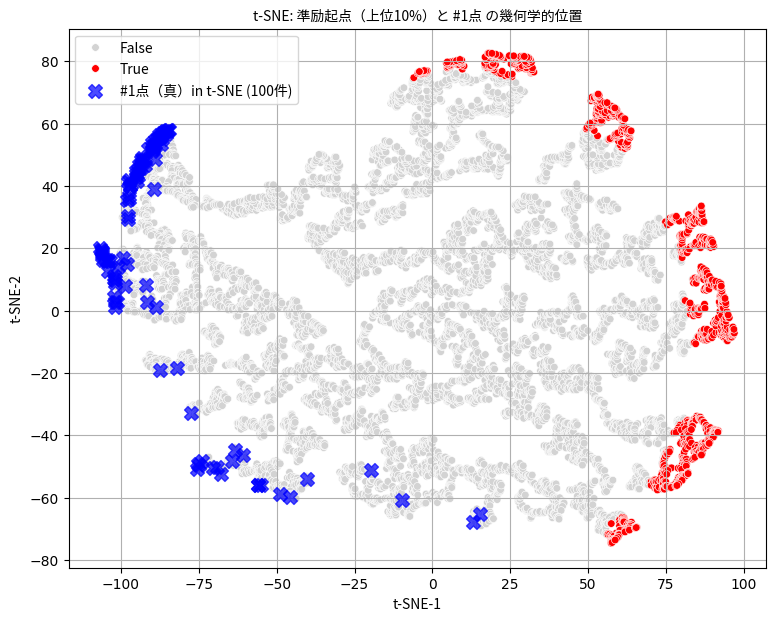
\includegraphics[width=0.8\linewidth]{S1_tsne_projection_robustness.png}
    \caption{Result of 2D projection via t-SNE. Red dots indicate quasi-excited points, and blue 'X' markers indicate \#1 points. The clear clustering of quasi-excited points and the localization of \#1 points within or near these clusters are distinctly observed, which is qualitatively consistent with the results from UMAP.}
    \label{fig:supp_tsne_projection}
\end{figure}

As Fig.~\ref{fig:supp_tsne_projection} shows, the quasi-excited points (red dots) are not randomly distributed but form multiple clusters. Furthermore, most of the \#1 points (blue 'X' markers) are located in positions strongly correlated with these quasi-excited point clusters. The consistent observation of this primary geometric feature across both UMAP and t-SNE provides strong evidence that this structure is an intrinsic property of the data.

\subsection*{S1.2. Universality of Dynamic Synchronization: FFT Analysis in Multiple Regions}
\label{subsec:supp_fft}

Next, we investigated whether the dynamic synchronization between indicators is a universal feature by extracting data sequences from four candidate regions (Regions 1--4) identified in the t-SNE space (Fig.~\ref{fig:supp_tsne_projection}), which show characteristic distributions of quasi-excited points and \#1 points. Each sequence was sorted in ascending order of the corresponding info-potential values before performing FFT analysis.

Figure~\ref{fig:supp_fft_regions} displays the FFT spectra of the three indicators (info-potential, $\mathrm{d}c/\mathrm{d}t$, and $\kappa(p)$) for each of the four candidate regions. The dominant frequencies and phases obtained from each analysis are summarized in Table~\ref{tab:supp_fft_peak_results}.

\begin{figure}[H]
    \centering
    \begin{subfigure}{0.48\linewidth}
        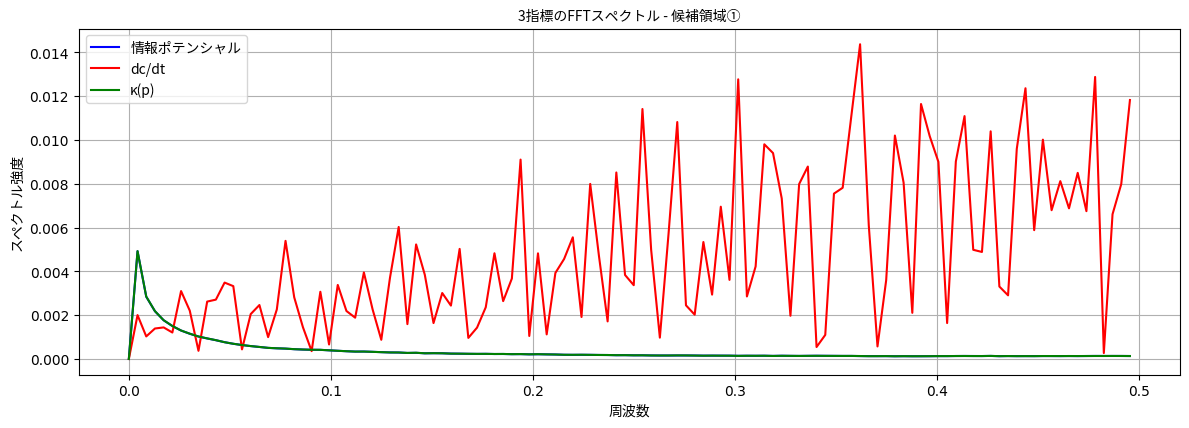
\includegraphics[width=\linewidth]{S1_fft_spectre_seq1.png}
        \caption{FFT spectra for Candidate Region 1.}
        \label{fig:supp_fft_region1}
    \end{subfigure}
    \hfill
    \begin{subfigure}{0.48\linewidth}
        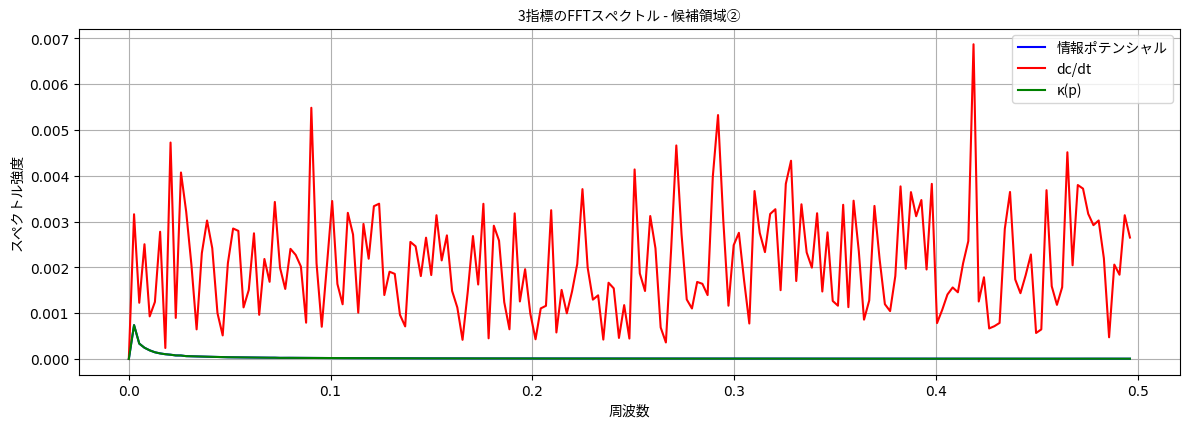
\includegraphics[width=\linewidth]{S1_fft_spectre_seq2.png}
        \caption{FFT spectra for Candidate Region 2.}
        \label{fig:supp_fft_region2}
    \end{subfigure}
    \vspace{1cm}
    \begin{subfigure}{0.48\linewidth}
        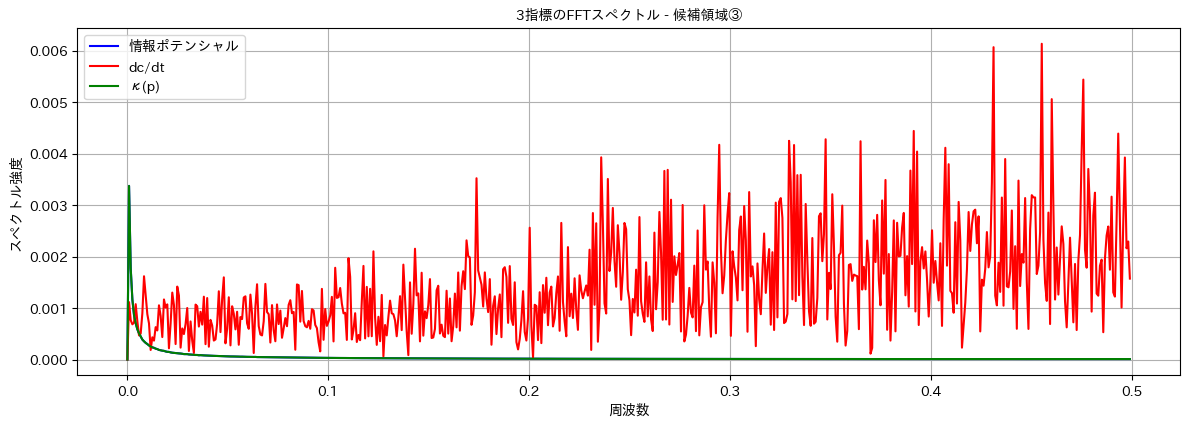
\includegraphics[width=\linewidth]{S1_fft_spectre_seq3.png}
        \caption{FFT spectra for Candidate Region 3.}
        \label{fig:supp_fft_region3}
    \end{subfigure}
    \hfill
    \begin{subfigure}{0.48\linewidth}
        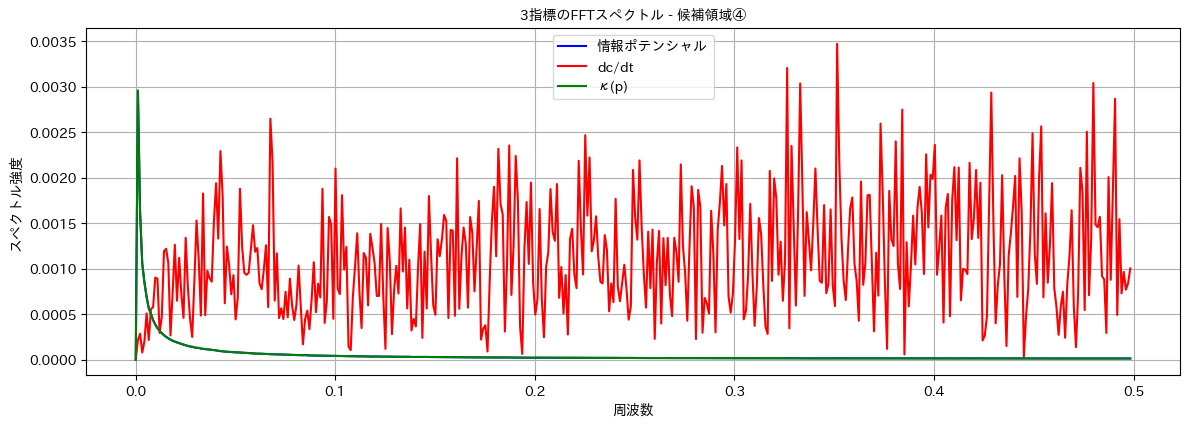
\includegraphics[width=\linewidth]{S1_fft_spectre_seq4.png}
        \caption{FFT spectra for Candidate Region 4.}
        \label{fig:supp_fft_region4}
    \end{subfigure}
    \caption{FFT spectra of the three indicators for sequences extracted from four different candidate regions.}
    \label{fig:supp_fft_regions}
\end{figure}

\begin{table}[H]
    \centering
    \caption{Dominant frequencies and phases of the three indicators in each candidate region.}
    \label{tab:supp_fft_peak_results}
    \begin{tabular}{@{}lccc@{}}
        \toprule
        \textbf{Candidate Region} & \textbf{Indicator} & \textbf{Dominant Freq.} & \textbf{Phase [deg]} \\
        \midrule
        \textbf{Region 1} & Info-potential & 0.0043 & 105.25 \\
                         & $\mathrm{d}c/\mathrm{d}t$ & 0.3621 & 106.76 \\
                         & $\kappa(p)$ & 0.0043 & 105.27 \\
        \midrule
        \textbf{Region 2} & Info-potential & 0.0026 & 92.35 \\
                         & $\mathrm{d}c/\mathrm{d}t$ & 0.4186 & 40.17 \\
                         & $\kappa(p)$ & 0.0026 & 92.35 \\
        \midrule
        \textbf{Region 3} & Info-potential & 0.0008 & 94.59 \\
                         & $\mathrm{d}c/\mathrm{d}t$ & 0.4553 & 41.32 \\
                         & $\kappa(p)$ & 0.0008 & 94.59 \\
        \midrule
        \textbf{Region 4} & Info-potential & 0.0011 & 98.46 \\
                         & $\mathrm{d}c/\mathrm{d}t$ & 0.3515 & -144.86 \\
                         & $\kappa(p)$ & 0.0011 & 98.46 \\
        \bottomrule
    \end{tabular}
\end{table}

As Table~\ref{tab:supp_fft_peak_results} clearly shows, in all four analyzed regions, the info-potential and $\kappa(p)$ exhibit a common, very low dominant frequency with a phase difference of nearly zero. This strongly suggests that the dynamic synchronization, where these two indicators are strongly coupled and oscillate in phase in a specific low-frequency mode, is not a local phenomenon but a universal feature in structures associated with \#1 points.

\subsection*{S1.3. Hierarchical Synchronization: Response at the Dominant Frequency of $\mathrm{d}c/\mathrm{d}t$}
\label{subsec:supp_hierarchical_sync}

In §S1.2, it was suggested that while the info-potential and $\kappa(p)$ synchronize at low frequencies, $\mathrm{d}c/\mathrm{d}t$ exhibits a hierarchical dynamic, dominating at a different, higher frequency. To investigate this further, we evaluated how the other two indicators respond at the dominant frequency of $\mathrm{d}c/\mathrm{d}t$.

We re-evaluated the spectral intensity and phase of the info-potential and $\kappa(p)$ at the target frequency corresponding to the dominant frequency of $\mathrm{d}c/\mathrm{d}t$ for each of Candidate Regions 1 and 2. The results are shown in Fig.~\ref{fig:supp_fft_re_regions} and Table~\ref{tab:supp_fft_re_results}.

\begin{figure}[H]
    \centering
    \begin{subfigure}{0.48\linewidth}
        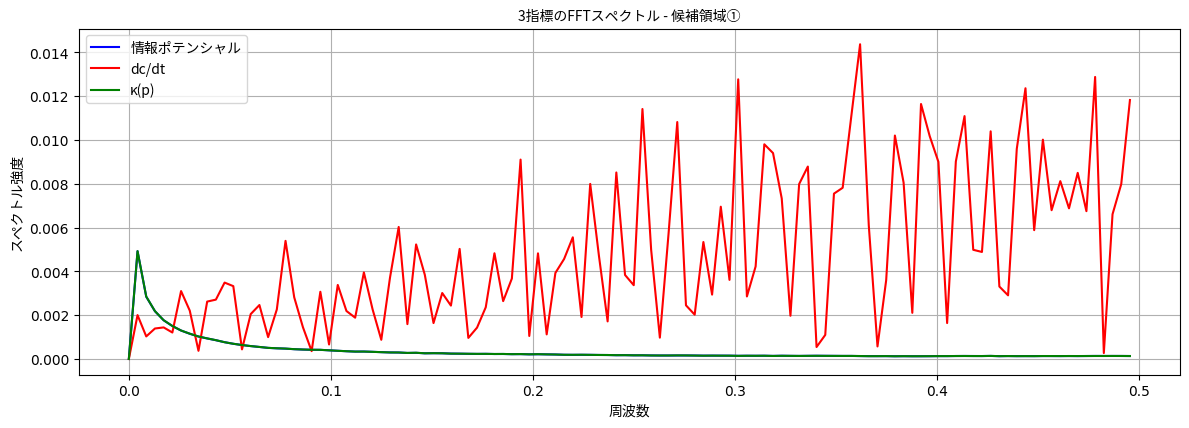
\includegraphics[width=\linewidth]{S1_fft_spectre_seq1.png}
        \caption{Region 1 (Targeting $\mathrm{d}c/\mathrm{d}t$ Freq.)}
        \label{fig:supp_fft_region1_re}
    \end{subfigure}
    \hfill
    \begin{subfigure}{0.48\linewidth}
        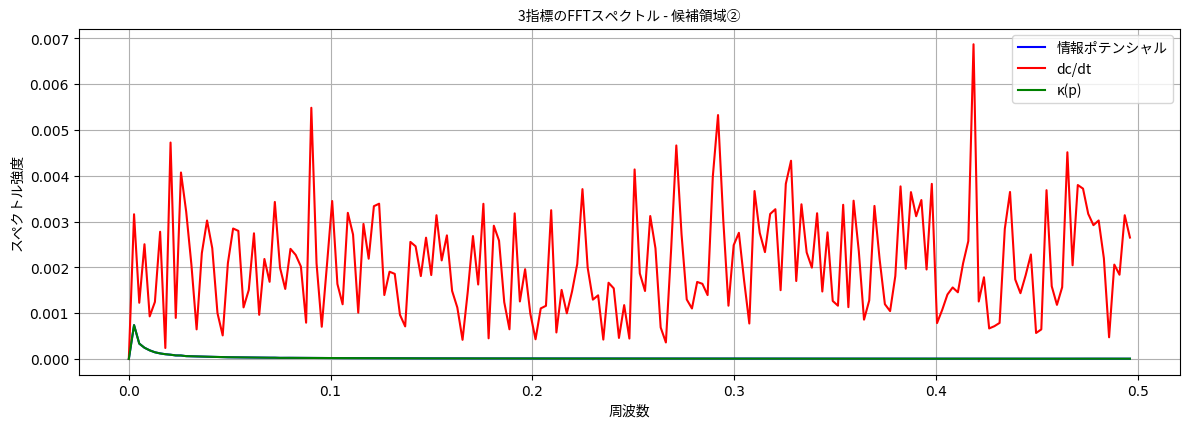
\includegraphics[width=\linewidth]{S1_fft_spectre_seq2.png}
        \caption{Region 2 (Targeting $\mathrm{d}c/\mathrm{d}t$ Freq.)}
        \label{fig:supp_fft_region2_re}
    \end{subfigure}
    \caption{FFT spectra of the three indicators for Candidate Regions 1 and 2, targeting the dominant frequency of $\mathrm{d}c/\mathrm{d}t$ in each region.}
    \label{fig:supp_fft_re_regions}
\end{figure}

\begin{table}[H]
    \centering
    \caption{Response of each indicator at the dominant frequency of $\mathrm{d}c/\mathrm{d}t$.}
    \label{tab:supp_fft_re_results}
    \begin{tabular}{@{}lccc@{}}
        \toprule
        \textbf{Region @ Target Freq.} & \textbf{Indicator} & \textbf{Intensity [a.u.]} & \textbf{Phase [deg]} \\
        \midrule
        \textbf{Region 1 @ 0.3621 Hz} & Info-potential & $1.32 \times 10^{-4}$ & 154.32 \\
                         & $\mathrm{d}c/\mathrm{d}t$ & $1.44 \times 10^{-2}$ & 106.76 \\
                         & $\kappa(p)$ & $1.35 \times 10^{-4}$ & 154.32 \\
        \midrule
        \textbf{Region 2 @ 0.4186 Hz} & Info-potential & $6.10 \times 10^{-6}$ & 166.76 \\
                         & $\mathrm{d}c/\mathrm{d}t$ & $6.87 \times 10^{-3}$ & 40.17 \\
                         & $\kappa(p)$ & $6.12 \times 10^{-6}$ & 166.51 \\
        \bottomrule
    \end{tabular}
\end{table}

As shown in Table~\ref{tab:supp_fft_re_results}, at the dominant frequency of $\mathrm{d}c/\mathrm{d}t$, the spectral intensities of the info-potential and $\kappa(p)$ are more than two orders of magnitude smaller than that of $\mathrm{d}c/\mathrm{d}t$ itself. However, these two indicators respond almost perfectly in phase with each other (phase difference of 0.00° in Region 1 and 0.25° in Region 2).

This result suggests that the info-potential and $\kappa(p)$, which describe the fundamental state of the system, respond in unison even to the higher-frequency "perturbations" induced by $\mathrm{d}c/\mathrm{d}t$. This, combined with the strong synchronization at low frequencies, underpins the hierarchical and stable dynamic properties of the "vortex phase" structure.


\section*{S2. Details of the Cosmological Validation}
\label{sec:supp_cosmological_validation}

This section details the intermediate analysis steps that led to the final joint analysis results presented in the main paper.

\subsection*{S2.1. Parameter Estimation from SNe Ia Data Alone}
\label{subsec:supp_sne_only_fit}

As the first step in constraining the DIRT Quadrupole model, we performed an MCMC analysis using only the full 1701 Type Ia supernovae data from the Pantheon+ catalog.

Figure~\ref{fig:supp_mcmc_sne_only} shows the posterior probability distributions for each parameter obtained from this SNe-only analysis. The median values and 1-sigma (68\%) confidence intervals are listed below.

\begin{figure}[H]
    \centering
    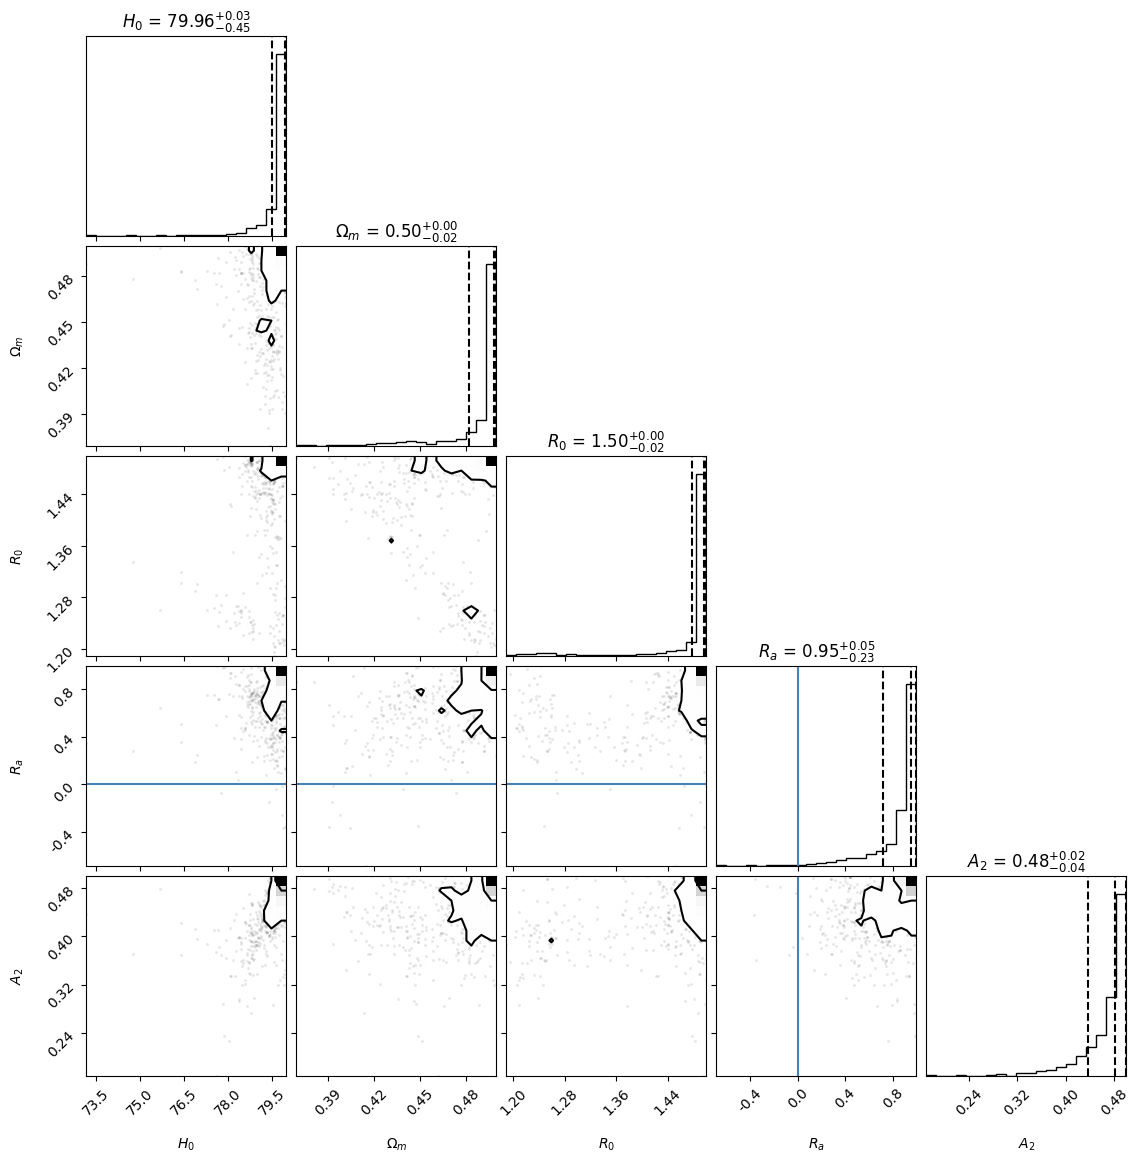
\includegraphics[width=\linewidth]{S2_MCMC_analysis_of_SNe_Ia_alone.png}
    \caption{Corner plot of the parameters obtained from the MCMC analysis using only SNe Ia data.}
    \label{fig:supp_mcmc_sne_only}
\end{figure}

\begin{itemize}
    \item $H_0 = 79.958 ^{+0.034} _{-0.448}$ km/s/Mpc
    \item $\Omega_m = 0.499 ^{+0.001} _{-0.017}$
    \item $R_0 = 1.497 ^{+0.003} _{-0.019}$
    \item $R_a = 0.951 ^{+0.047} _{-0.229}$
    \item $A_2 = 0.481 ^{+0.018} _{-0.044}$
\end{itemize}

This result indicates that the SNe Ia data strongly favor a model with a large anisotropy amplitude ($A_2 \approx 0.48$). However, it also shows that other fundamental cosmological parameters, such as $H_0$ and $\Omega_m$, deviate significantly from the values estimated by the standard $\Lambda$CDM model. This suggests the necessity of verifying whether this model is consistent with other observations, which motivates the comparison with BAO data and the final joint analysis.

\subsection*{S2.2. The Role of BAO Data and Comparison with the Joint Analysis}
\label{subsec:supp_joint_comparison}

The SNe-only analysis strongly suggested a large anisotropy $A_2$. This section examines how this result changed with the addition of BAO data in the joint analysis and discusses the role of BAO data in constraining our model parameters.

Table~\ref{tab:supp_param_comparison} compares the best-fit parameters and their 1-sigma confidence intervals from the SNe-only analysis and the SNe+BAO joint analysis (see §4 of the main paper).

\begin{table}[H]
    \centering
    \caption{Comparison of parameter estimations from SNe-only and SNe+BAO joint analyses.}
    \label{tab:supp_param_comparison}
    \begin{tabular}{@{}lcc@{}}
        \toprule
        \textbf{Parameter} & \textbf{SNe-only (1701 points)} & \textbf{SNe+BAO (Joint Analysis)} \\
        \midrule
        $H_0$ [km/s/Mpc] & $79.958 ^{+0.034} _{-0.448}$ & $79.956 ^{+0.034} _{-0.148}$ \\
        $\Omega_m$ & $0.499 ^{+0.001} _{-0.017}$ & $0.499 ^{+0.001} _{-0.004}$ \\
        $R_0$ & $1.497 ^{+0.003} _{-0.019}$ & $1.198 ^{+0.002} _{-0.008}$ \\
        $R_a$ & $0.951 ^{+0.047} _{-0.229}$ & $0.981 ^{+0.016} _{-0.090}$ \\
        $A_2$ & $0.481 ^{+0.018} _{-0.044}$ & $0.488 ^{+0.011} _{-0.064}$ \\
        \bottomrule
    \end{tabular}
\end{table}

This comparison reveals several key points:
\begin{enumerate}
    \item \textbf{Robustness of the Anisotropy $A_2$}: This is the most crucial finding. Even with the addition of BAO data, which provides very strong constraints on the cosmic expansion history, the best-fit value of the anisotropy amplitude $A_2$ remains almost unchanged at $\approx 0.48$, and its confidence interval still does not include zero. This indicates that the anisotropy signal found in the SNe Ia data is not an artifact but a robust feature that is consistent with BAO data.
    \item \textbf{Readjustment of $R_0$}: The most significant shift occurred in $R_0$, the present-day value of the isotropic component of $R_{lock}$. While the SNe-only analysis preferred a large value of $\approx 1.5$, the joint analysis shifted it eTo $\approx 1.2$. This can be interpreted as the model "readjusting" its internal parameters to satisfy both the stringent expansion history required by BAO and the anisotropy required by SNe. The model found an exquisite balance point by lowering the value of $R_0$ to improve the fit to BAO data while maintaining a large $A_2$.
    \item \textbf{Improved Constraints on Other Parameters}: The error bars for parameters like $H_0$, $\Omega_m$, and $R_a$ were significantly reduced in the joint analysis. This demonstrates that combining different probes like SNe and BAO is effective at breaking degeneracies between parameters and substantially improving the overall constraints on the model.
\end{enumerate}

Overall, this comparison further strengthens the validity of our DIRT Quadrupole model. Far from refuting the existence of anisotropy, the BAO data contributed to determining the model's internal parameter values more precisely, supporting an anisotropic cosmological picture consistent with both SNe and BAO with high confidence.

\section*{S3. Proposal for Experimental Verification (Checklist ②)}
\label{sec:supp_experimental_proposal}

To physically establish the theoretical and observational results of this research, especially the importance of the Information Lock Coefficient $R_{lock}$, direct verification at the laboratory scale is essential. This section proposes a concrete plan for such a tabletop optical experiment.

\subsection*{S3.1. Experimental Concept and Objective}
\label{subsec:supp_exp_concept}

The objective of this experiment is to actively control the Information Lock Coefficient $R_{lock}$ over the range from 0 to 1 and to observe whether the "inertial" or "effective mass $m_{eff}$" aspect of a physical system transitions continuously, as predicted by DIRT theory. This verification is crucial for demonstrating the physical reality of $R_{lock}$ and the dynamic continuity between information, mass, and energy.

\subsection*{S3.2. Definition and Experimental Control of $R_{lock}$}
\label{subsec:supp_exp_rlock_control}

This experiment will use the fundamental equation for the Information Lock Coefficient defined in Paper D.
\begin{equation}
    R_{lock} = \frac{\tau_{det}}{\tau_{det}+\tau_{path}}\,(1-\beta_{scat})
    \label{eq:supp_rlock_experimental}
\end{equation}
Initially, we assume an ideal vacuum system with no scattering ($\beta_{scat} \approx 0$), aiming to control $R_{lock} \approx \tau_{det} / (\tau_{det}+\tau_{path})$. The parameters $\tau_{path}$ (photon propagation time) and $\tau_{det}$ (detection and information-confirmation time) will be independently controlled using a variable optical fiber delay line and a post-detection variable electronic delay module, respectively. This two-stage scanning strategy aims to experimentally cover the full operational range of $R_{lock}$.

\subsection*{S3.3. Proposed Experimental Setup and Measurands}
\label{subsec:supp_exp_setup_measurement}

The main components of the proposed experimental setup are illustrated in the conceptual diagram in Fig.~\ref{fig:supp_exp_setup_schematic}.

\begin{figure}[H]
    \centering
    \fbox{\parbox{0.8\linewidth}{\centering \vspace{5cm} (A conceptual diagram of the experimental setup will be inserted here, including: a light source, variable optical delay line, MEMS mirror, interferometer, SNSPD, and variable electronic delay.) \vspace{5cm}}}
    \caption{A conceptual diagram of the proposed tabletop optical experiment (image).}
    \label{fig:supp_exp_setup_schematic}
\end{figure}

\begin{itemize}
    \item \textbf{Light Source}: A picosecond pulsed laser (e.g., at 1550 nm) attenuated to the single-photon level.
    \item \textbf{$R_{lock}$ Control System}: The aforementioned variable optical fiber delay line (for $\tau_{path}$ control) and variable electronic delay module (for $\tau_{det}$ control).
    \item \textbf{Inertial Probe}: A high-Q MEMS cantilever or thin-film mirror that undergoes minute displacement upon momentum transfer from a light pulse (radiation pressure).
    \item \textbf{Displacement Detection System}: A high-sensitivity optical interferometer to read out the minute displacement of the MEMS mirror.
    \item \textbf{Photon Detector}: An SNSPD to record the arrival time of photons with high precision and to serve as a trigger/synchronization for the entire experiment.
\end{itemize}

The primary physical quantity to be measured is the momentum transfer from radiation pressure on the MEMS mirror. Specifically, by measuring the impulse (momentum $p$) or the response characteristics of the system, we will define a proxy for the "effective mass $m_{eff}$" or "inertial indicator." By plotting this proxy against $R_{lock}$, we aim to create a continuous transition curve of $m_{eff}(R_{lock})$.

DIRT theory predicts a continuous transition where $m_{eff} \to 0$ in the energy-dominant limit ($R_{lock} \to 0$) and $m_{eff}$ saturates to a finite value in the mass-dominant limit ($R_{lock} \to 1$). The final goal of this experiment is to compare this experimental curve with the theoretical prediction.

\end{document}